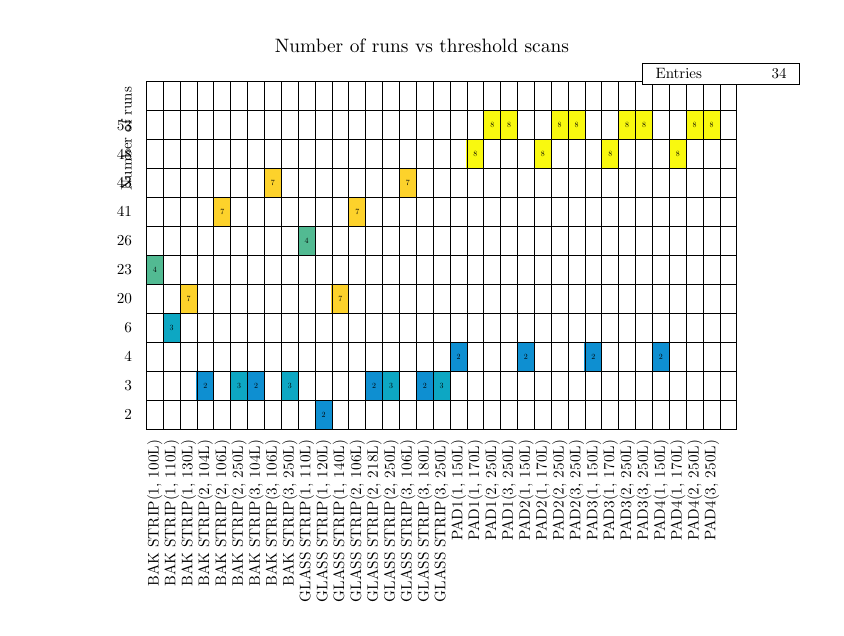
\begin{tikzpicture}
\pgfdeclareplotmark{cross} {
\pgfpathmoveto{\pgfpoint{-0.3\pgfplotmarksize}{\pgfplotmarksize}}
\pgfpathlineto{\pgfpoint{+0.3\pgfplotmarksize}{\pgfplotmarksize}}
\pgfpathlineto{\pgfpoint{+0.3\pgfplotmarksize}{0.3\pgfplotmarksize}}
\pgfpathlineto{\pgfpoint{+1\pgfplotmarksize}{0.3\pgfplotmarksize}}
\pgfpathlineto{\pgfpoint{+1\pgfplotmarksize}{-0.3\pgfplotmarksize}}
\pgfpathlineto{\pgfpoint{+0.3\pgfplotmarksize}{-0.3\pgfplotmarksize}}
\pgfpathlineto{\pgfpoint{+0.3\pgfplotmarksize}{-1.\pgfplotmarksize}}
\pgfpathlineto{\pgfpoint{-0.3\pgfplotmarksize}{-1.\pgfplotmarksize}}
\pgfpathlineto{\pgfpoint{-0.3\pgfplotmarksize}{-0.3\pgfplotmarksize}}
\pgfpathlineto{\pgfpoint{-1.\pgfplotmarksize}{-0.3\pgfplotmarksize}}
\pgfpathlineto{\pgfpoint{-1.\pgfplotmarksize}{0.3\pgfplotmarksize}}
\pgfpathlineto{\pgfpoint{-0.3\pgfplotmarksize}{0.3\pgfplotmarksize}}
\pgfpathclose
\pgfusepathqstroke
}
\pgfdeclareplotmark{cross*} {
\pgfpathmoveto{\pgfpoint{-0.3\pgfplotmarksize}{\pgfplotmarksize}}
\pgfpathlineto{\pgfpoint{+0.3\pgfplotmarksize}{\pgfplotmarksize}}
\pgfpathlineto{\pgfpoint{+0.3\pgfplotmarksize}{0.3\pgfplotmarksize}}
\pgfpathlineto{\pgfpoint{+1\pgfplotmarksize}{0.3\pgfplotmarksize}}
\pgfpathlineto{\pgfpoint{+1\pgfplotmarksize}{-0.3\pgfplotmarksize}}
\pgfpathlineto{\pgfpoint{+0.3\pgfplotmarksize}{-0.3\pgfplotmarksize}}
\pgfpathlineto{\pgfpoint{+0.3\pgfplotmarksize}{-1.\pgfplotmarksize}}
\pgfpathlineto{\pgfpoint{-0.3\pgfplotmarksize}{-1.\pgfplotmarksize}}
\pgfpathlineto{\pgfpoint{-0.3\pgfplotmarksize}{-0.3\pgfplotmarksize}}
\pgfpathlineto{\pgfpoint{-1.\pgfplotmarksize}{-0.3\pgfplotmarksize}}
\pgfpathlineto{\pgfpoint{-1.\pgfplotmarksize}{0.3\pgfplotmarksize}}
\pgfpathlineto{\pgfpoint{-0.3\pgfplotmarksize}{0.3\pgfplotmarksize}}
\pgfpathclose
\pgfusepathqfillstroke
}
\pgfdeclareplotmark{newstar} {
\pgfpathmoveto{\pgfqpoint{0pt}{\pgfplotmarksize}}
\pgfpathlineto{\pgfqpointpolar{44}{0.5\pgfplotmarksize}}
\pgfpathlineto{\pgfqpointpolar{18}{\pgfplotmarksize}}
\pgfpathlineto{\pgfqpointpolar{-20}{0.5\pgfplotmarksize}}
\pgfpathlineto{\pgfqpointpolar{-54}{\pgfplotmarksize}}
\pgfpathlineto{\pgfqpointpolar{-90}{0.5\pgfplotmarksize}}
\pgfpathlineto{\pgfqpointpolar{234}{\pgfplotmarksize}}
\pgfpathlineto{\pgfqpointpolar{198}{0.5\pgfplotmarksize}}
\pgfpathlineto{\pgfqpointpolar{162}{\pgfplotmarksize}}
\pgfpathlineto{\pgfqpointpolar{134}{0.5\pgfplotmarksize}}
\pgfpathclose
\pgfusepathqstroke
}
\pgfdeclareplotmark{newstar*} {
\pgfpathmoveto{\pgfqpoint{0pt}{\pgfplotmarksize}}
\pgfpathlineto{\pgfqpointpolar{44}{0.5\pgfplotmarksize}}
\pgfpathlineto{\pgfqpointpolar{18}{\pgfplotmarksize}}
\pgfpathlineto{\pgfqpointpolar{-20}{0.5\pgfplotmarksize}}
\pgfpathlineto{\pgfqpointpolar{-54}{\pgfplotmarksize}}
\pgfpathlineto{\pgfqpointpolar{-90}{0.5\pgfplotmarksize}}
\pgfpathlineto{\pgfqpointpolar{234}{\pgfplotmarksize}}
\pgfpathlineto{\pgfqpointpolar{198}{0.5\pgfplotmarksize}}
\pgfpathlineto{\pgfqpointpolar{162}{\pgfplotmarksize}}
\pgfpathlineto{\pgfqpointpolar{134}{0.5\pgfplotmarksize}}
\pgfpathclose
\pgfusepathqfillstroke
}
\definecolor{c}{rgb}{1,1,1};
\draw [color=c, fill=c] (0,0) rectangle (10,6.79083);
\draw [color=c, fill=c] (1.5,1.69771) rectangle (9,6.11175);
\definecolor{c}{rgb}{0,0,0};
\draw [c,line width=0.3] (1.5,1.69771) -- (1.5,6.11175) -- (9,6.11175) -- (9,1.69771) -- (1.5,1.69771);
\definecolor{c}{rgb}{0.0557375,0.560081,0.819366};
\draw [color=c, fill=c] (3.64286,1.69771) rectangle (3.85714,2.06554);
\draw [color=c, fill=c] (2.14286,2.06554) rectangle (2.35714,2.43338);
\definecolor{c}{rgb}{0.0526375,0.656131,0.763481};
\draw [color=c, fill=c] (2.57143,2.06554) rectangle (2.78571,2.43338);
\definecolor{c}{rgb}{0.0557375,0.560081,0.819366};
\draw [color=c, fill=c] (2.78571,2.06554) rectangle (3,2.43338);
\definecolor{c}{rgb}{0.0526375,0.656131,0.763481};
\draw [color=c, fill=c] (3.21429,2.06554) rectangle (3.42857,2.43338);
\definecolor{c}{rgb}{0.0557375,0.560081,0.819366};
\draw [color=c, fill=c] (4.28571,2.06554) rectangle (4.5,2.43338);
\definecolor{c}{rgb}{0.0526375,0.656131,0.763481};
\draw [color=c, fill=c] (4.5,2.06554) rectangle (4.71429,2.43338);
\definecolor{c}{rgb}{0.0557375,0.560081,0.819366};
\draw [color=c, fill=c] (4.92857,2.06554) rectangle (5.14286,2.43338);
\definecolor{c}{rgb}{0.0526375,0.656131,0.763481};
\draw [color=c, fill=c] (5.14286,2.06554) rectangle (5.35714,2.43338);
\definecolor{c}{rgb}{0.0557375,0.560081,0.819366};
\draw [color=c, fill=c] (5.35714,2.43338) rectangle (5.57143,2.80122);
\draw [color=c, fill=c] (6.21429,2.43338) rectangle (6.42857,2.80122);
\draw [color=c, fill=c] (7.07143,2.43338) rectangle (7.28571,2.80122);
\draw [color=c, fill=c] (7.92857,2.43338) rectangle (8.14286,2.80122);
\definecolor{c}{rgb}{0.0526375,0.656131,0.763481};
\draw [color=c, fill=c] (1.71429,2.80122) rectangle (1.92857,3.16905);
\definecolor{c}{rgb}{0.992,0.823138,0.170006};
\draw [color=c, fill=c] (1.92857,3.16905) rectangle (2.14286,3.53689);
\draw [color=c, fill=c] (3.85714,3.16905) rectangle (4.07143,3.53689);
\definecolor{c}{rgb}{0.322347,0.730556,0.570878};
\draw [color=c, fill=c] (1.5,3.53689) rectangle (1.71429,3.90473);
\draw [color=c, fill=c] (3.42857,3.90473) rectangle (3.64286,4.27256);
\definecolor{c}{rgb}{0.992,0.823138,0.170006};
\draw [color=c, fill=c] (2.35714,4.27256) rectangle (2.57143,4.6404);
\draw [color=c, fill=c] (4.07143,4.27256) rectangle (4.28571,4.6404);
\draw [color=c, fill=c] (3,4.6404) rectangle (3.21429,5.00824);
\draw [color=c, fill=c] (4.71429,4.6404) rectangle (4.92857,5.00824);
\definecolor{c}{rgb}{0.977,0.977044,0.0583656};
\draw [color=c, fill=c] (5.57143,5.00824) rectangle (5.78571,5.37607);
\draw [color=c, fill=c] (6.42857,5.00824) rectangle (6.64286,5.37607);
\draw [color=c, fill=c] (7.28571,5.00824) rectangle (7.5,5.37607);
\draw [color=c, fill=c] (8.14286,5.00824) rectangle (8.35714,5.37607);
\draw [color=c, fill=c] (5.78571,5.37607) rectangle (6,5.74391);
\draw [color=c, fill=c] (6,5.37607) rectangle (6.21429,5.74391);
\draw [color=c, fill=c] (6.64286,5.37607) rectangle (6.85714,5.74391);
\draw [color=c, fill=c] (6.85714,5.37607) rectangle (7.07143,5.74391);
\draw [color=c, fill=c] (7.5,5.37607) rectangle (7.71429,5.74391);
\draw [color=c, fill=c] (7.71429,5.37607) rectangle (7.92857,5.74391);
\draw [color=c, fill=c] (8.35714,5.37607) rectangle (8.57143,5.74391);
\draw [color=c, fill=c] (8.57143,5.37607) rectangle (8.78571,5.74391);
\definecolor{c}{rgb}{0,0,0};
\draw [c,line width=0.3] (1.5,1.69771) -- (9,1.69771);
\draw [anchor= east] (1.60714,1.6315) node[scale=0.55, color=c,rotate=90]{BAK STRIP(1, 100L)};
\draw [anchor= east] (1.82143,1.6315) node[scale=0.55, color=c,rotate=90]{BAK STRIP(1, 110L)};
\draw [anchor= east] (2.03571,1.6315) node[scale=0.55, color=c,rotate=90]{BAK STRIP(1, 130L)};
\draw [anchor= east] (2.25,1.6315) node[scale=0.55, color=c,rotate=90]{BAK STRIP(2, 104L)};
\draw [anchor= east] (2.46429,1.6315) node[scale=0.55, color=c,rotate=90]{BAK STRIP(2, 106L)};
\draw [anchor= east] (2.67857,1.6315) node[scale=0.55, color=c,rotate=90]{BAK STRIP(2, 250L)};
\draw [anchor= east] (2.89286,1.6315) node[scale=0.55, color=c,rotate=90]{BAK STRIP(3, 104L)};
\draw [anchor= east] (3.10714,1.6315) node[scale=0.55, color=c,rotate=90]{BAK STRIP(3, 106L)};
\draw [anchor= east] (3.32143,1.6315) node[scale=0.55, color=c,rotate=90]{BAK STRIP(3, 250L)};
\draw [anchor= east] (3.53571,1.6315) node[scale=0.55, color=c,rotate=90]{GLASS STRIP(1, 110L)};
\draw [anchor= east] (3.75,1.6315) node[scale=0.55, color=c,rotate=90]{GLASS STRIP(1, 120L)};
\draw [anchor= east] (3.96429,1.6315) node[scale=0.55, color=c,rotate=90]{GLASS STRIP(1, 140L)};
\draw [anchor= east] (4.17857,1.6315) node[scale=0.55, color=c,rotate=90]{GLASS STRIP(2, 106L)};
\draw [anchor= east] (4.39286,1.6315) node[scale=0.55, color=c,rotate=90]{GLASS STRIP(2, 218L)};
\draw [anchor= east] (4.60714,1.6315) node[scale=0.55, color=c,rotate=90]{GLASS STRIP(2, 250L)};
\draw [anchor= east] (4.82143,1.6315) node[scale=0.55, color=c,rotate=90]{GLASS STRIP(3, 106L)};
\draw [anchor= east] (5.03571,1.6315) node[scale=0.55, color=c,rotate=90]{GLASS STRIP(3, 180L)};
\draw [anchor= east] (5.25,1.6315) node[scale=0.55, color=c,rotate=90]{GLASS STRIP(3, 250L)};
\draw [anchor= east] (5.46429,1.6315) node[scale=0.55, color=c,rotate=90]{PAD1(1, 150L)};
\draw [anchor= east] (5.67857,1.6315) node[scale=0.55, color=c,rotate=90]{PAD1(1, 170L)};
\draw [anchor= east] (5.89286,1.6315) node[scale=0.55, color=c,rotate=90]{PAD1(2, 250L)};
\draw [anchor= east] (6.10714,1.6315) node[scale=0.55, color=c,rotate=90]{PAD1(3, 250L)};
\draw [anchor= east] (6.32143,1.6315) node[scale=0.55, color=c,rotate=90]{PAD2(1, 150L)};
\draw [anchor= east] (6.53571,1.6315) node[scale=0.55, color=c,rotate=90]{PAD2(1, 170L)};
\draw [anchor= east] (6.75,1.6315) node[scale=0.55, color=c,rotate=90]{PAD2(2, 250L)};
\draw [anchor= east] (6.96429,1.6315) node[scale=0.55, color=c,rotate=90]{PAD2(3, 250L)};
\draw [anchor= east] (7.17857,1.6315) node[scale=0.55, color=c,rotate=90]{PAD3(1, 150L)};
\draw [anchor= east] (7.39286,1.6315) node[scale=0.55, color=c,rotate=90]{PAD3(1, 170L)};
\draw [anchor= east] (7.60714,1.6315) node[scale=0.55, color=c,rotate=90]{PAD3(2, 250L)};
\draw [anchor= east] (7.82143,1.6315) node[scale=0.55, color=c,rotate=90]{PAD3(3, 250L)};
\draw [anchor= east] (8.03571,1.6315) node[scale=0.55, color=c,rotate=90]{PAD4(1, 150L)};
\draw [anchor= east] (8.25,1.6315) node[scale=0.55, color=c,rotate=90]{PAD4(1, 170L)};
\draw [anchor= east] (8.46429,1.6315) node[scale=0.55, color=c,rotate=90]{PAD4(2, 250L)};
\draw [anchor= east] (8.67857,1.6315) node[scale=0.55, color=c,rotate=90]{PAD4(3, 250L)};
\draw [c,line width=0.3] (1.5,1.8505) -- (1.5,1.69771);
\draw [c,line width=0.3] (1.5,6.11175) -- (1.5,1.69771);
\draw [c,line width=0.3] (1.71429,1.8505) -- (1.71429,1.69771);
\draw [c,line width=0.3] (1.71429,6.11175) -- (1.71429,1.69771);
\draw [c,line width=0.3] (1.92857,1.8505) -- (1.92857,1.69771);
\draw [c,line width=0.3] (1.92857,6.11175) -- (1.92857,1.69771);
\draw [c,line width=0.3] (2.14286,1.8505) -- (2.14286,1.69771);
\draw [c,line width=0.3] (2.14286,6.11175) -- (2.14286,1.69771);
\draw [c,line width=0.3] (2.35714,1.8505) -- (2.35714,1.69771);
\draw [c,line width=0.3] (2.35714,6.11175) -- (2.35714,1.69771);
\draw [c,line width=0.3] (2.57143,1.8505) -- (2.57143,1.69771);
\draw [c,line width=0.3] (2.57143,6.11175) -- (2.57143,1.69771);
\draw [c,line width=0.3] (2.78571,1.8505) -- (2.78571,1.69771);
\draw [c,line width=0.3] (2.78571,6.11175) -- (2.78571,1.69771);
\draw [c,line width=0.3] (3,1.8505) -- (3,1.69771);
\draw [c,line width=0.3] (3,6.11175) -- (3,1.69771);
\draw [c,line width=0.3] (3.21429,1.8505) -- (3.21429,1.69771);
\draw [c,line width=0.3] (3.21429,6.11175) -- (3.21429,1.69771);
\draw [c,line width=0.3] (3.42857,1.8505) -- (3.42857,1.69771);
\draw [c,line width=0.3] (3.42857,6.11175) -- (3.42857,1.69771);
\draw [c,line width=0.3] (3.64286,1.8505) -- (3.64286,1.69771);
\draw [c,line width=0.3] (3.64286,6.11175) -- (3.64286,1.69771);
\draw [c,line width=0.3] (3.85714,1.8505) -- (3.85714,1.69771);
\draw [c,line width=0.3] (3.85714,6.11175) -- (3.85714,1.69771);
\draw [c,line width=0.3] (4.07143,1.8505) -- (4.07143,1.69771);
\draw [c,line width=0.3] (4.07143,6.11175) -- (4.07143,1.69771);
\draw [c,line width=0.3] (4.28571,1.8505) -- (4.28571,1.69771);
\draw [c,line width=0.3] (4.28571,6.11175) -- (4.28571,1.69771);
\draw [c,line width=0.3] (4.5,1.8505) -- (4.5,1.69771);
\draw [c,line width=0.3] (4.5,6.11175) -- (4.5,1.69771);
\draw [c,line width=0.3] (4.71429,1.8505) -- (4.71429,1.69771);
\draw [c,line width=0.3] (4.71429,6.11175) -- (4.71429,1.69771);
\draw [c,line width=0.3] (4.92857,1.8505) -- (4.92857,1.69771);
\draw [c,line width=0.3] (4.92857,6.11175) -- (4.92857,1.69771);
\draw [c,line width=0.3] (5.14286,1.8505) -- (5.14286,1.69771);
\draw [c,line width=0.3] (5.14286,6.11175) -- (5.14286,1.69771);
\draw [c,line width=0.3] (5.35714,1.8505) -- (5.35714,1.69771);
\draw [c,line width=0.3] (5.35714,6.11175) -- (5.35714,1.69771);
\draw [c,line width=0.3] (5.57143,1.8505) -- (5.57143,1.69771);
\draw [c,line width=0.3] (5.57143,6.11175) -- (5.57143,1.69771);
\draw [c,line width=0.3] (5.78571,1.8505) -- (5.78571,1.69771);
\draw [c,line width=0.3] (5.78571,6.11175) -- (5.78571,1.69771);
\draw [c,line width=0.3] (6,1.8505) -- (6,1.69771);
\draw [c,line width=0.3] (6,6.11175) -- (6,1.69771);
\draw [c,line width=0.3] (6.21429,1.8505) -- (6.21429,1.69771);
\draw [c,line width=0.3] (6.21429,6.11175) -- (6.21429,1.69771);
\draw [c,line width=0.3] (6.42857,1.8505) -- (6.42857,1.69771);
\draw [c,line width=0.3] (6.42857,6.11175) -- (6.42857,1.69771);
\draw [c,line width=0.3] (6.64286,1.8505) -- (6.64286,1.69771);
\draw [c,line width=0.3] (6.64286,6.11175) -- (6.64286,1.69771);
\draw [c,line width=0.3] (6.85714,1.8505) -- (6.85714,1.69771);
\draw [c,line width=0.3] (6.85714,6.11175) -- (6.85714,1.69771);
\draw [c,line width=0.3] (7.07143,1.8505) -- (7.07143,1.69771);
\draw [c,line width=0.3] (7.07143,6.11175) -- (7.07143,1.69771);
\draw [c,line width=0.3] (7.28571,1.8505) -- (7.28571,1.69771);
\draw [c,line width=0.3] (7.28571,6.11175) -- (7.28571,1.69771);
\draw [c,line width=0.3] (7.5,1.8505) -- (7.5,1.69771);
\draw [c,line width=0.3] (7.5,6.11175) -- (7.5,1.69771);
\draw [c,line width=0.3] (7.71429,1.8505) -- (7.71429,1.69771);
\draw [c,line width=0.3] (7.71429,6.11175) -- (7.71429,1.69771);
\draw [c,line width=0.3] (7.92857,1.8505) -- (7.92857,1.69771);
\draw [c,line width=0.3] (7.92857,6.11175) -- (7.92857,1.69771);
\draw [c,line width=0.3] (8.14286,1.8505) -- (8.14286,1.69771);
\draw [c,line width=0.3] (8.14286,6.11175) -- (8.14286,1.69771);
\draw [c,line width=0.3] (8.35714,1.8505) -- (8.35714,1.69771);
\draw [c,line width=0.3] (8.35714,6.11175) -- (8.35714,1.69771);
\draw [c,line width=0.3] (8.57143,1.8505) -- (8.57143,1.69771);
\draw [c,line width=0.3] (8.57143,6.11175) -- (8.57143,1.69771);
\draw [c,line width=0.3] (8.78571,1.8505) -- (8.78571,1.69771);
\draw [c,line width=0.3] (8.78571,6.11175) -- (8.78571,1.69771);
\draw [c,line width=0.3] (9,1.8505) -- (9,1.69771);
\draw [c,line width=0.3] (9,6.11175) -- (9,1.69771);
\draw [c,line width=0.3] (1.5,1.69771) -- (1.5,6.11175);
\draw [anchor= east] (1.3875,1.88163) node[scale=0.55, color=c, rotate=0]{ 2};
\draw [anchor= east] (1.3875,2.24946) node[scale=0.55, color=c, rotate=0]{ 3};
\draw [anchor= east] (1.3875,2.6173) node[scale=0.55, color=c, rotate=0]{ 4};
\draw [anchor= east] (1.3875,2.98514) node[scale=0.55, color=c, rotate=0]{ 6};
\draw [anchor= east] (1.3875,3.35297) node[scale=0.55, color=c, rotate=0]{20};
\draw [anchor= east] (1.3875,3.72081) node[scale=0.55, color=c, rotate=0]{23};
\draw [anchor= east] (1.3875,4.08865) node[scale=0.55, color=c, rotate=0]{26};
\draw [anchor= east] (1.3875,4.45648) node[scale=0.55, color=c, rotate=0]{41};
\draw [anchor= east] (1.3875,4.82432) node[scale=0.55, color=c, rotate=0]{43};
\draw [anchor= east] (1.3875,5.19216) node[scale=0.55, color=c, rotate=0]{48};
\draw [anchor= east] (1.3875,5.55999) node[scale=0.55, color=c, rotate=0]{53};
\draw [c,line width=0.3] (1.695,1.69771) -- (1.5,1.69771);
\draw [c,line width=0.3] (9,1.69771) -- (1.5,1.69771);
\draw [c,line width=0.3] (1.695,2.06554) -- (1.5,2.06554);
\draw [c,line width=0.3] (9,2.06554) -- (1.5,2.06554);
\draw [c,line width=0.3] (1.695,2.43338) -- (1.5,2.43338);
\draw [c,line width=0.3] (9,2.43338) -- (1.5,2.43338);
\draw [c,line width=0.3] (1.695,2.80122) -- (1.5,2.80122);
\draw [c,line width=0.3] (9,2.80122) -- (1.5,2.80122);
\draw [c,line width=0.3] (1.695,3.16905) -- (1.5,3.16905);
\draw [c,line width=0.3] (9,3.16905) -- (1.5,3.16905);
\draw [c,line width=0.3] (1.695,3.53689) -- (1.5,3.53689);
\draw [c,line width=0.3] (9,3.53689) -- (1.5,3.53689);
\draw [c,line width=0.3] (1.695,3.90473) -- (1.5,3.90473);
\draw [c,line width=0.3] (9,3.90473) -- (1.5,3.90473);
\draw [c,line width=0.3] (1.695,4.27256) -- (1.5,4.27256);
\draw [c,line width=0.3] (9,4.27256) -- (1.5,4.27256);
\draw [c,line width=0.3] (1.695,4.6404) -- (1.5,4.6404);
\draw [c,line width=0.3] (9,4.6404) -- (1.5,4.6404);
\draw [c,line width=0.3] (1.695,5.00824) -- (1.5,5.00824);
\draw [c,line width=0.3] (9,5.00824) -- (1.5,5.00824);
\draw [c,line width=0.3] (1.695,5.37607) -- (1.5,5.37607);
\draw [c,line width=0.3] (9,5.37607) -- (1.5,5.37607);
\draw [c,line width=0.3] (1.695,5.74391) -- (1.5,5.74391);
\draw [c,line width=0.3] (9,5.74391) -- (1.5,5.74391);
\draw [c,line width=0.3] (1.695,6.11175) -- (1.5,6.11175);
\draw [c,line width=0.3] (9,6.11175) -- (1.5,6.11175);
\draw [anchor= east] (1.24785,6.11175) node[scale=0.540924, color=c, rotate=90]{Number of runs};
\definecolor{c}{rgb}{1,1,1};
\draw [color=c, fill=c] (7.8,6.07779) rectangle (9.8,6.34943);
\definecolor{c}{rgb}{0,0,0};
\draw [c,line width=0.3] (7.8,6.07779) -- (9.8,6.07779);
\draw [c,line width=0.3] (9.8,6.07779) -- (9.8,6.34943);
\draw [c,line width=0.3] (9.8,6.34943) -- (7.8,6.34943);
\draw [c,line width=0.3] (7.8,6.34943) -- (7.8,6.07779);
\draw [anchor= west] (7.9,6.21361) node[scale=0.540924, color=c, rotate=0]{Entries };
\draw [anchor= east] (9.7,6.21361) node[scale=0.540924, color=c, rotate=0]{ 34};
\definecolor{c}{rgb}{1,1,1};
\draw [color=c, fill=c] (7.8,6.07779) rectangle (9.8,6.34943);
\definecolor{c}{rgb}{0,0,0};
\draw [c,line width=0.3] (7.8,6.07779) -- (9.8,6.07779);
\draw [c,line width=0.3] (9.8,6.07779) -- (9.8,6.34943);
\draw [c,line width=0.3] (9.8,6.34943) -- (7.8,6.34943);
\draw [c,line width=0.3] (7.8,6.34943) -- (7.8,6.07779);
\draw [anchor= west] (7.9,6.21361) node[scale=0.540924, color=c, rotate=0]{Entries };
\draw [anchor= east] (9.7,6.21361) node[scale=0.540924, color=c, rotate=0]{ 34};
\definecolor{c}{rgb}{1,1,1};
\draw [color=c, fill=c] (7.8,6.07779) rectangle (9.8,6.34943);
\definecolor{c}{rgb}{0,0,0};
\draw [c,line width=0.3] (7.8,6.07779) -- (9.8,6.07779);
\draw [c,line width=0.3] (9.8,6.07779) -- (9.8,6.34943);
\draw [c,line width=0.3] (9.8,6.34943) -- (7.8,6.34943);
\draw [c,line width=0.3] (7.8,6.34943) -- (7.8,6.07779);
\draw [anchor= west] (7.9,6.21361) node[scale=0.540924, color=c, rotate=0]{Entries };
\draw [anchor= east] (9.7,6.21361) node[scale=0.540924, color=c, rotate=0]{ 34};
\draw (3.75,1.88163) node[scale=0.286371, color=c, rotate=0]{2};
\draw (2.25,2.24946) node[scale=0.286371, color=c, rotate=0]{2};
\draw (2.67857,2.24946) node[scale=0.286371, color=c, rotate=0]{3};
\draw (2.89286,2.24946) node[scale=0.286371, color=c, rotate=0]{2};
\draw (3.32143,2.24946) node[scale=0.286371, color=c, rotate=0]{3};
\draw (4.39286,2.24946) node[scale=0.286371, color=c, rotate=0]{2};
\draw (4.60714,2.24946) node[scale=0.286371, color=c, rotate=0]{3};
\draw (5.03571,2.24946) node[scale=0.286371, color=c, rotate=0]{2};
\draw (5.25,2.24946) node[scale=0.286371, color=c, rotate=0]{3};
\draw (5.46429,2.6173) node[scale=0.286371, color=c, rotate=0]{2};
\draw (6.32143,2.6173) node[scale=0.286371, color=c, rotate=0]{2};
\draw (7.17857,2.6173) node[scale=0.286371, color=c, rotate=0]{2};
\draw (8.03571,2.6173) node[scale=0.286371, color=c, rotate=0]{2};
\draw (1.82143,2.98514) node[scale=0.286371, color=c, rotate=0]{3};
\draw (2.03571,3.35297) node[scale=0.286371, color=c, rotate=0]{7};
\draw (3.96429,3.35297) node[scale=0.286371, color=c, rotate=0]{7};
\draw (1.60714,3.72081) node[scale=0.286371, color=c, rotate=0]{4};
\draw (3.53571,4.08865) node[scale=0.286371, color=c, rotate=0]{4};
\draw (2.46429,4.45648) node[scale=0.286371, color=c, rotate=0]{7};
\draw (4.17857,4.45648) node[scale=0.286371, color=c, rotate=0]{7};
\draw (3.10714,4.82432) node[scale=0.286371, color=c, rotate=0]{7};
\draw (4.82143,4.82432) node[scale=0.286371, color=c, rotate=0]{7};
\draw (5.67857,5.19216) node[scale=0.286371, color=c, rotate=0]{8};
\draw (6.53571,5.19216) node[scale=0.286371, color=c, rotate=0]{8};
\draw (7.39286,5.19216) node[scale=0.286371, color=c, rotate=0]{8};
\draw (8.25,5.19216) node[scale=0.286371, color=c, rotate=0]{8};
\draw (5.89286,5.55999) node[scale=0.286371, color=c, rotate=0]{8};
\draw (6.10714,5.55999) node[scale=0.286371, color=c, rotate=0]{8};
\draw (6.75,5.55999) node[scale=0.286371, color=c, rotate=0]{8};
\draw (6.96429,5.55999) node[scale=0.286371, color=c, rotate=0]{8};
\draw (7.60714,5.55999) node[scale=0.286371, color=c, rotate=0]{8};
\draw (7.82143,5.55999) node[scale=0.286371, color=c, rotate=0]{8};
\draw (8.46429,5.55999) node[scale=0.286371, color=c, rotate=0]{8};
\draw (8.67857,5.55999) node[scale=0.286371, color=c, rotate=0]{8};
\definecolor{c}{rgb}{1,1,1};
\draw [color=c, fill=c] (7.8,6.07779) rectangle (9.8,6.34943);
\definecolor{c}{rgb}{0,0,0};
\draw [c,line width=0.3] (7.8,6.07779) -- (9.8,6.07779);
\draw [c,line width=0.3] (9.8,6.07779) -- (9.8,6.34943);
\draw [c,line width=0.3] (9.8,6.34943) -- (7.8,6.34943);
\draw [c,line width=0.3] (7.8,6.34943) -- (7.8,6.07779);
\draw [anchor= west] (7.9,6.21361) node[scale=0.540924, color=c, rotate=0]{Entries };
\draw [anchor= east] (9.7,6.21361) node[scale=0.540924, color=c, rotate=0]{ 34};
\draw (5,6.57013) node[scale=0.700019, color=c, rotate=0]{Number of runs vs threshold scans};
\end{tikzpicture}
